% Created 2024-03-02 sáb 11:26
% Intended LaTeX compiler: pdflatex
\documentclass[bigger]{beamer}
\usepackage[utf8]{inputenc}
\usepackage[T1]{fontenc}
\usepackage{graphicx}
\usepackage{longtable}
\usepackage{wrapfig}
\usepackage{rotating}
\usepackage[normalem]{ulem}
\usepackage{amsmath}
\usepackage{amssymb}
\usepackage{capt-of}
\usepackage{hyperref}
\mode<beamer>{\usetheme{Madrid}}
\usetheme{default}
\author{Adrián Arroyo Calle}
\date{Curso 2023-2024}
\title{Memoria compartida}
\hypersetup{
 pdfauthor={Adrián Arroyo Calle},
 pdftitle={Memoria compartida},
 pdfkeywords={},
 pdfsubject={},
 pdfcreator={Emacs 29.2 (Org mode 9.6.15)}, 
 pdflang={Spanish}}
\begin{document}

\maketitle

\section{Memoria compartida}
\label{sec:org675ff0d}

\begin{frame}[label={sec:org0744647}]{¿Qué es?}
\begin{itemize}
\item La ley de Moore nos dice que acada 18 meses duplicamos el número de transistores.
\item Podíamos usar esos transistores para aumentar la frecuencia, pero cada vez más difícil
\item Podemos usar los transistores en \emph{núcleos} adicionales
\item Idea muy popular: prácticamente todos los procesadores actuales son multinúcleo
\end{itemize}
\end{frame}

\begin{frame}[label={sec:org59987c0}]{Intel Core i7 3960X}
\begin{center}
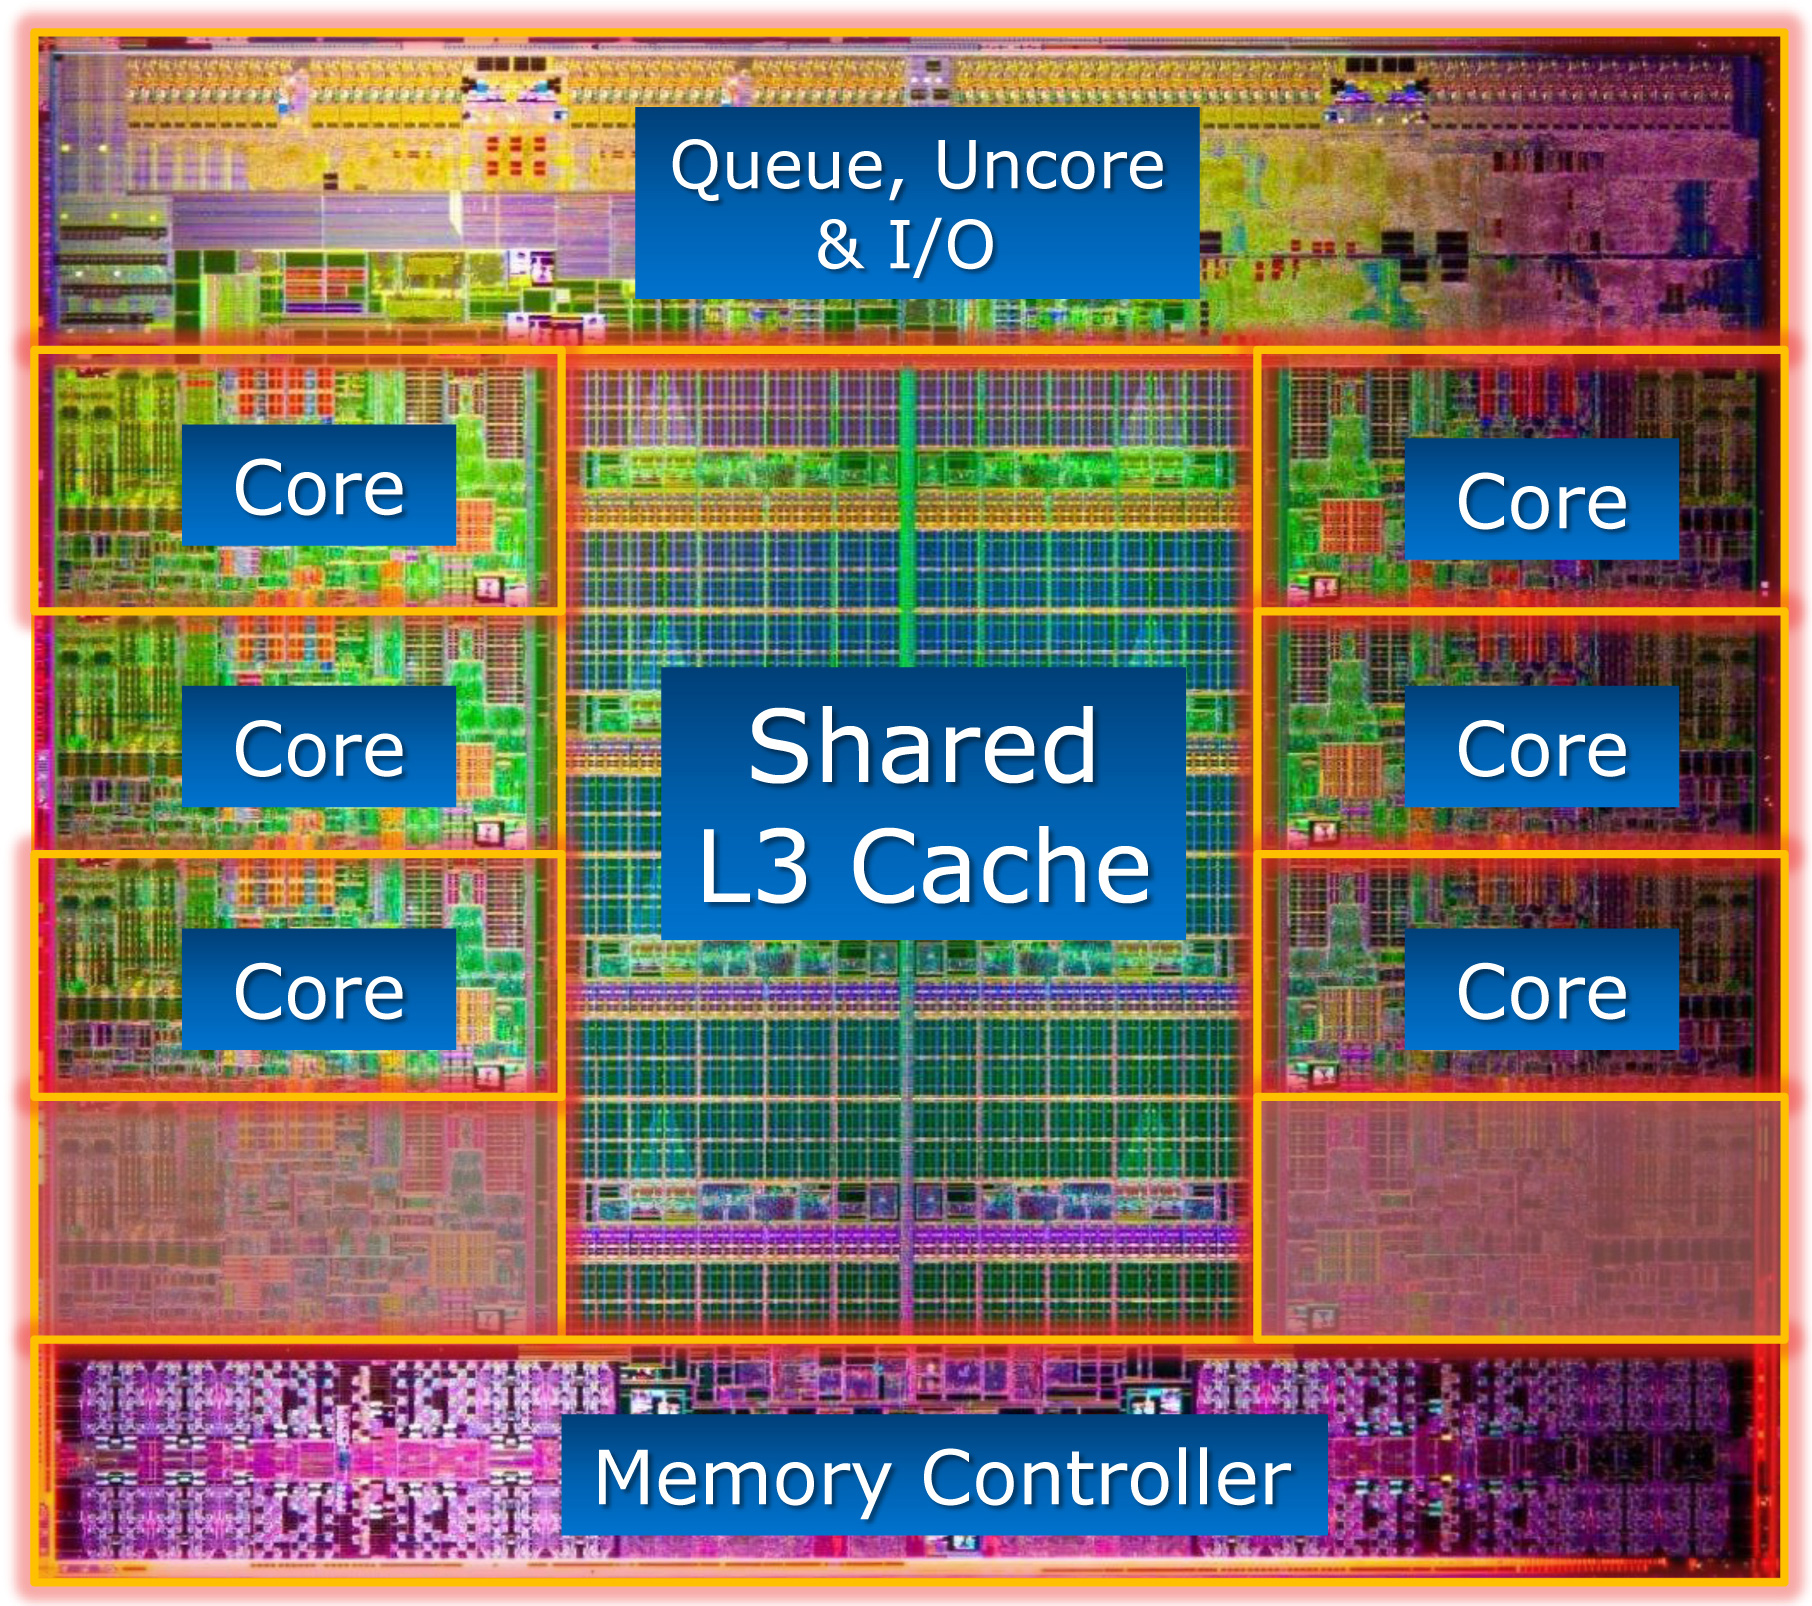
\includegraphics[width=0.8\textwidth]{./IntelCorei7Die.jpg}
\end{center}
\end{frame}

\begin{frame}[label={sec:orgde9bdc5}]{Núcleos separados, memoria unificada}
\begin{itemize}
\item Arquitectura Von Neumman: código y datos en la misma memoria
\item Los núcleos van leyendo de memoria las instrucciones, y las ejecutan de forma \alert{independiente} (control y aritmética).
\item Habrá instrucciones que modifiquen el estado de la memoria.
\item La memoria para todos los núcleos es la misma.
\item Así pues los núcleos son independientes, pero \alert{comparten la misma memoria} (comparten código y datos)
\end{itemize}
\end{frame}

\begin{frame}[label={sec:orgcdb8a72}]{Pros y contras}
Pros

\begin{itemize}
\item Solución relativamente barata
\item Al compartir memoria, no hay que copiar datos, lo que mejora el rendimiento
\end{itemize}

Contras

\begin{itemize}
\item Escalabilidad reducida. Los procesadores multinúcleo tienen un límite de núcleos por diseño.
\item Sincronización. Es fácil que dos núcleos operen sobre los mismos datos y generen problemas de sincronización.
\end{itemize}
\end{frame}

\begin{frame}[label={sec:org7e4c37a}]{¿Cómo se consigue?}
\begin{itemize}
\item Las primitivas necesarias nos las tiene que ofrecer el sistema operativo.
\item Una solución muy popular es \emph{POSIX Threads} (\emph{pthreads})
\begin{itemize}
\item Es nativo en Linux, macOS, Android, FreeBSD, Solaris, AIX, \ldots{}
\item Pero NO es nativo en Windows
\end{itemize}
\item Para algunos casos muy comunes en supercomputación existe un estándar: OpenMP
\item Se basa en directivas (comentarios) que se añaden al código C, C++ o FORTRAN.
\end{itemize}
\end{frame}

\begin{frame}[label={sec:org6d63ba3}]{A alto nivel}
\begin{itemize}
\item los lenguajes de más alto nivel, como Julia, suelen implementar su propia API similar a OpenMP.
\item Por debajo se implementan usando \emph{pthreads} u otra API del sistema operativo
\end{itemize}
\end{frame}

\begin{frame}[label={sec:orgbd0ec08},fragile]{Julia}
 \begin{block}{Consultar número de threads}
\begin{verbatim}
julia
julia> Threads.nthreads()
1
\end{verbatim}

\begin{itemize}
\item Por defecto Julia se lanza solo con un thread habilitado
\end{itemize}
\end{block}

\begin{block}{Ajustar número de threads}
\begin{verbatim}
julia --threads=auto
julia> Threads.nthreads()
4
\end{verbatim}

\begin{itemize}
\item Con el parámetro threads podemos ajustar los threads iniciales
\item \texttt{auto} intentará adivinar el número óptimo de threads. También podemos pasar un número entero.
\end{itemize}
\end{block}
\end{frame}

\begin{frame}[label={sec:orgb9808a4},fragile]{Número de threads}
 \begin{itemize}
\item ¿Cuál es el número máximo de threads que puedo meter?
\begin{itemize}
\item El límite lo pone el sistema operativo. Podemos tener miles de threads.
\end{itemize}
\item El sistema operativo (el scheduler) \alert{reparte} los threads entre los núcleos.
\begin{itemize}
\item En Linux hay varios schedulers a elegir y todos son muy configurables.
\end{itemize}
\item Pero no es efectivo tener más threads que núcleos.
\begin{itemize}
\item A maś threads, más coste de sincronización. Pero si no hay núcleos para respaldarlos, no se paraleliza.
\item El número ideal es \alert{tantos threads como núcleos tengamos} (lo que hace \texttt{auto})
\end{itemize}
\end{itemize}
\end{frame}

\begin{frame}[label={sec:org4e83749},fragile]{Macro @spawn}
 \begin{block}{Macro @spawn}
\begin{verbatim}
julia> function f()
           print(Threads.threadid())
       end
julia> task = Threads.@spawn f()
\end{verbatim}

\begin{itemize}
\item Con la macro \texttt{@spawn} creamos un \texttt{Task} que se ejecuta una función en un thread.
\end{itemize}
\end{block}
\end{frame}

\begin{frame}[label={sec:org825a3a5},fragile]{Macro @spawn}
 \begin{block}{Macro @spawn con wait}
\begin{verbatim}
julia> t() = println("Hola desde ", Threads.threadid())
julia> tasks = wait.([Threads.@spawn t() for i in 1:4])
Hola desde 3
Hola desde 4
Hola desde 2
Hola desde 1
\end{verbatim}
\begin{itemize}
\item Sobre la task podemos hacer \texttt{wait} para esperar a que acabe, o \texttt{fetch} para además guardar sus resultados en un vector.
\end{itemize}
\end{block}
\end{frame}


\begin{frame}[label={sec:org35cb32f},fragile]{Macro @spawn}
 \begin{block}{Macro @spawn con fetch}
\begin{verbatim}
julia> t() = Threads.threadid()
julia> fetch.([Threads.@spawn t() for i in 1:4])
4-element Vector{Int64}:
 1
 2
 3
 4
\end{verbatim}
\end{block}
\end{frame}

\begin{frame}[label={sec:orgfbe6852},fragile]{Macro @threads}
 \begin{block}{Macro @threads}
\begin{verbatim}
julia> Threads.@threads for i in 1:10
           println(Threads.threadid())
       end
1214344312
\end{verbatim}

\begin{itemize}
\item La macro \texttt{@threads} nos permite paralelizar un bucle for.
\end{itemize}
\end{block}
\end{frame}
\end{document}
